% -*- mode: latex-mode; TeX-engine: xetex; LaTeX-command-style: (("" "SOURCE_DATE_EPOCH=0 %(PDF)%(latex) --shell-escape %S%(PDFout)")); TeX-master: "../dissertation.tex"; -*-

\chapter{Introduction}
\label{ch:introduction}

\section{Ultracold Molecules}
\label{ch:introduction:molecules}

Started with precise optical spectroscopy and the development of laser cooling
and trapping technologies, the increasing measurement precision and
high level of control has been one of the the primary driving forces
in the field of atomic physics in the past decades.
Systems based on cooling and controlling of neutral atoms
have been used in a wide range of applications including
quantum computing, quantum communication, precision measurement,
quantum simulation and the study of many other many body effects.

Despite these great successes, the utility of atom based systems
are limited by their simple internal structure and weak interactions.
Molecules, on the other hand, with its richer internal degrees of freedom
including electronic orbital, electron spin, neuclear vibration, rotation and spin,
the potential of stronger interaction and more variance of symmetry classes,
are better candidates for more applications especially in
precision measurement~\cite{kondov_molecular_2019,kozyryev_precision_2017,
  flambaum_electric_2020,acme_collaboration_improved_2018,cairncross_precision_2017,
  hudson_improved_2011},
quantum simulations~\cite{micheli_toolbox_2006,yao_quantum_2018,
  wall_quantum_2015,wall_realizing_2015},
quantum information processing~\cite{demille_quantum_2002,ni_dipolar_2018,
  hudson_dipolar_2018,lin_quantum_2020},
and quantum chemistry~\cite{balakrishnan_perspective_2016,hu_direct_2019,
  segev_collisions_2019,jongh_imaging_2020}.
Moreover, comparing to other systems with stronger interaction like ions and Rydberg atoms,
the interacting states in molecules are long lived and tunable thanks to
the abundance of low energy excitations,
which can offer better isolation from the environment giving rise to longer coherence time.

Many applications of molecules requires cooling and high level of control
on the quantum state of the molecules.
Unfortunately, the properties that makes molecules attractive
also makes controlling them harder.
The enabling technique for most ultracold atom experiment, laser cooling,
typically requires scattering of a large number of photons ($\approx10^4\sim10^8$).
This is possible in atomic system due to the existence of cycling transition
or near cycling ones that can be completely closed with
one or two spin states repumping lasers.
However, the lack of selection rules for vibrational states means that
such transition generally does not exist in molecules.
As a result, experiments aiming to achieve control of molecule on a similar level with atoms
usually take one of the two approaches,
\begin{enumerate}
\item Direct laser cooling of special molecules
  with approximate cycling transitions~\cite{norrgard_submillikelvin_2016,
    anderegg_laser_2018,mitra_direct_2020,ding_sub-doppler_2020,
    mccarron_magnetic_2018,truppe_molecules_2017}.\\
  These are molecules that have optical transitions that has a high probability
  of decaying down to the same vibrational states.
  With the help of a few vibrational repumping lasers,
  scattering of $\approx10^3\sim10^7$ photons can be achieved.
  Significant progress has been made using this approach in recent years
  including sub-doppler cooling~\cite{cheuk_mathrmlambda-enhanced_2018}
  and trapping of molecules in optical tweezers~\cite{anderegg_optical_2019}.
  The main challenge with this approach is to achieve a better cooling performance
  given the still limitted photon scattering budget.
\item Creation of molecules from ultracold atoms.\\
  First realized a decade ago~\cite{ni_high_2008,lang_ultracold_2008},
  this approach takes advantage of the mature cooling and trapping techniques
  developped for atoms and creates molecules from atoms
  that are cooled to ultracold temperature.
  The difficulty with this approach is understandably in the creation of the molecule,
  which must be done with acceptable efficiency and coherence
  in order to maintain the cooling and controling done on the atoms.
  This approach currently allows a lower temperature to be achieved~\cite{
    marco_degenerate_2019,zhang_forming_2020,he_coherently_2020}
  and this is the approach used in our experiment.
\end{enumerate}

\section{Assembly of Molecules in Optical Tweezers}
\label{ch:introduction:tweezers}

Previous experiments that takes the approach to create ultracold molecules
from ultracold atoms do so either in a bulk gases or an optical lattice.
In these systems, however, the transfer efficiency and
the density of the created molecules are limited
by the overlap between the distribution of the two atomic speices.
Such overlap is controlled by the combination of the trapping potential
and the intra- and inter-species interactions.
Thus, a perfect overlap for molecule formation can only be achieved by fine tuning
the delicate balance between these parameters and may not always be possible.
Additionally, the molecules created in such matter may collide
with residue atoms or other molecules causing rapid loss
either through chemical reactions or by forming long-lived sticky complex.

Since these issues are essentially all caused by the lack of direct control
on the position and motion of individual atoms and molecules,
we propose a general solution using optical tweezers.
Created by focusing the trap light through a high numerical aperture~(NA) objective,
optical tweezers can trap single atoms in flexible geometry
and the setup naturally provides the high resolution required
for detection and manipulation of individual atoms~\cite{schlosser_sub-poissonian_2001}.
Taking advantage of these properties, full quantum control on atoms has been demostrated
by cooling and rearranging the tweezer based on the loading result.
This gives us a good starting point to deterministically create molecules
by directly merging pairs of atoms instead of
relying on stochastic process or the fine tuning of parameters in previous experiments.
The molecules created using this approach are also well isolated from each other,
preventing loss due to collisions.

\subsection{Two-Step All Optical Creation of Molecules}
\label{ch:introduction:tweezers:two-step}

In order to create the rovibronic ground state molecules from atoms,
the $\approx100~\mathrm{THz}$ binding energy must be removed coherently from the system,
which is may be done using a two-photon optical transition.
However, due to the significant mismatch in the wavefunction size
between the atomic motional ground state~($\approx1000\text{\AA}$)
and the rovibronic ground state of the molecule~($\approx4\text{\AA}$),
it is challenging to achieve a high Rabi frequency or short transition time,
causing technical difficulties in maintaining the laser coherence during the transition.
Because of this, the transfer to rovibronic ground state is typically done in two steps.
The atoms are first associated to a weakly bound molecule
where the coherence is easier to achieve due to the smaller energy difference.
After that the molecule can be driven to the rovibronic ground state more quickly,
relaxing the coherence requirement. See section~\ref{ch:raman-transfer:state-selction}
for a more detailed and systematic description of the challenges
and the selection of the transfer pathway.

So far, most experiments implemented the first step
by magnetoassociation using a magnetic Feshbach scattering resonance~\cite{
  ni_high_2008,zhang_forming_2020}.
The only exceptions are $\mathrm{Sr}_2$,
where narrow-linewidth ($\sim 20~\mathrm{kHz}$) excited states
are available and optical association can be driven coherently~\cite{
  reinaudi_optical_2012,stellmer_creation_2012}
and $^{87}\mathrm{Rb}^{85}\mathrm{Rb}$,
where there are molecular states bound by $1\sim2~\mathrm{MHz}$~\cite{he_coherently_2020}.
With these requirements, molecules involving non-magnetic atoms
or atoms without narrow intercombination lines remain difficult to associate.

In our experiment, we propose a different method using only optical transitions
and does not rely on an narrow excited state linewidth.
This is enabled by the confinement of the optical tweezer and
careful selection of the transition pathway,
which will be covered in more detail in later chapters.
We believe the approach we demostrate in our experiment is more general
than the previous ones,
and can be applied to most other molecules created from laser-coolable atoms.

\subsection{Experiment Plan}
\label{ch:introduction:tweezers:plan}

\begin{figure}
  \centering
  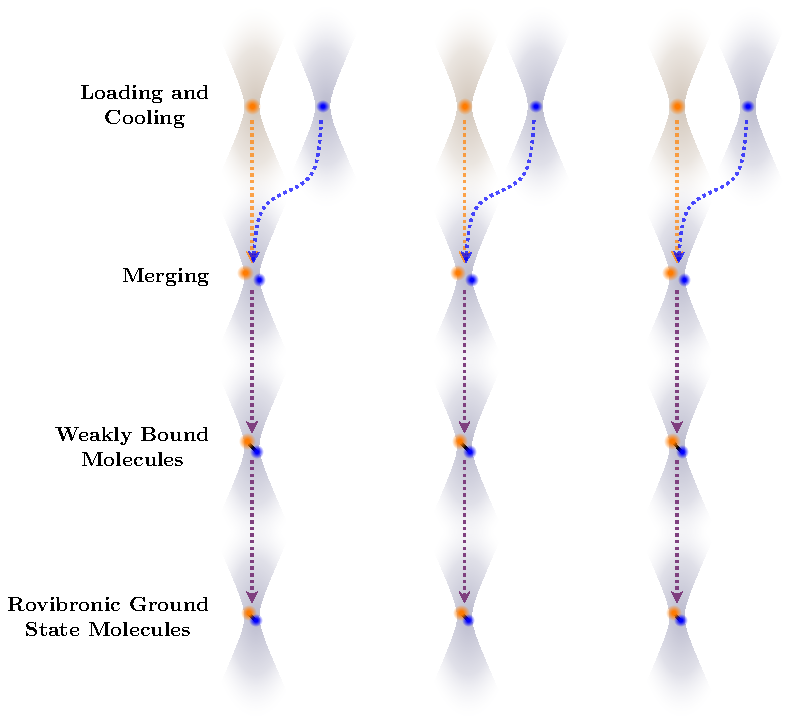
\includegraphics[width=\textwidth]{figures/introduction_steps.pdf}
  \caption[Molecule creation steps.]{
    Steps to create single rovibronic molecules in optical tweezers.
    \label{fig:introduction:tweezers:plan:steps}}
\end{figure}

The molecule we use to implement this approach is NaCs.
We selected a bialkali molecule in order to take advantage of
the wide range of existing techniques developped to cool and manipulate alkali atoms.
The molecule is also predicted to have a large
molecular fixed-frame dipole moments~($4.6~\mathrm{Debye}$)
in the singlet rovibronic ground state,
making it a good candidate to demostrate interaction and entanglement
after created in the tweezers.

The steps we propose to create the molecules in the tweezer are show in
Fig.~\ref{fig:introduction:tweezers:plan:steps} and are listed as follows,
\begin{enumerate}
\item Loading and cooling of single atoms in the tweezers.\\
  This is the step that give us the full quantum control on the atoms
  which will be translated to the control on the molecules later.
  Image of the atoms taken in this step can be used to rearrange the tweezers
  to acheive high filling fraction.
\item Merging of the atoms into a single tweezer.\\
  Using the precise control of the atoms from optical tweezers,
  we can merge a single Na and Cs that is trapped and cooled in separate tweezers
  into a single one deterministically.
\item Creation of weakly bound molecule.\\
  The pair of atoms in a single tweezer will be coherently associated
  to a weakly bound molecule using a Raman transition detuned from an excited molecular state.
  This is the critical step that transfers the control we achieved
  on the atoms to molecules and will be the main result of this thesis.
\item Creation of rovibronic ground state molecule.\\
  Finally, the weakly bound molecule will be driven to the rovibronic ground state
  using another two-photon transition.
  This prepare the molecule in a state with strong dipole interaction
  and can be used for many previously mentioned applications.
\end{enumerate}

\section{Contents of this Thesis}
\label{ch:introduction:contents}

In this thesis, we describe the method we use to create a weakly bound ground state molecule
in the optical tweezer and the results leading up to it including the control of atoms
and the measurement on the interaction between the atoms and the molecular potential.

We start with chapter \ref{ch:computer-control} by giving a high level description of
the custom computer control system we use.
This system controls the timing of all the hardware outputs in the experiment
and is used to perform all the measurements in the rest of this thesis.

Chapter \ref{ch:loading} discusses the loading of the single atoms into the optical tweezer.
The discussion includes the preparation steps needed before the loading,
e.g. freespace cooling of atoms,
and the imaging of the atom in the tweezer,
which is the primary detection method used in our experiment.
All the experiments in the following chapters are performed using
the atoms and molecules in the optical tweezers.

Chapter \ref{ch:rsc} describes the Raman sideband cooling (RSC) process
we used to cool single Na atom in the optical tweezer.
As the lighter atom with a broader optical linewidth,
the RSC of Na atom faces additional challenges compared to atoms
that were cooled using similar method previously
and the tool we developed to overcome these challenges can be applied to other systems as well.

After preparation of the atomic state,
chapter \ref{ch:interaction-shift} starts our investigation of the interaction between atoms
by measuring the $s$-wave scattering length using interaction shift spectroscopy.
The measurement result is used to refine the prediction for Feshbach resonance
between Na and Cs atoms and also to improve the atomic state preparation.

Chapter \ref{ch:pa} discusses the measurement of the molecular excited states
by photoassociation spectroscopy.
We also study the effect of the tweezer beam on the molecular states and transitions.
The states mapped out in this measurement are used as intermediate states
to study the groud molecular states via two-photon transitions.

Following the previous chapter, chapter \ref{ch:raman-spectroscopy} discusses
the properties of the weakly bound ground molecular states using Raman spectroscopy.
We demostrated the ability to control the rotational states of the molecule
and studies the coupling of the molecule with external field
and the their hyperfine structure in the weakly bound regime.
The measurement identifies candidate target states for our coherent molecule creation.

Chapter \ref{ch:raman-transfer} combines the preparation and characterization
in the previous chapters and describes our all-optical coherent molecule formation process.
A detailed comparison between different approaches and states selection is given
to support our choice of experimental parameters.
We show our result on the coherent transfer and characterizes
the molecule we create as well as the transfer process.
We study the limit on the transfer efficiency
and list open questions in the transfer process
as well as possible future improvements.
